%%%%%%%%%%%%%%%%%%%%%%%%%%%%%%%%%%%%%%%%%%%%%%%%%%%%%%%%%%%%%%%%%%%%%
\newpage
\hfill 24.06.
%%%%%%%%%%%%%%%%%%%%%%%%%%%%%%%%%%%%%%%%%%%%%%%%%%%%%%%%%%%%%%%%%%%%%

\section{Denotationelle Semantik}


\begin{remark}[Ziel]
    Die Definition einer semantischen Funktion direkt ohne Umweg über eine simulierte Programmausführung (\dh{} ohne eine Übergangsrelation).

    Dabei ist die Zusammengsetztheit (\emph{compositionality}) bei der Definition der semantischen Funktion für ein Sprachkonstrukt wichtig, \dh{} man darf nur die Werte der semantischen Funktion für die Bestandteile des Sprachkonstrukts verwenden.
\end{remark}

\begin{example}
    \[ \A: \AExp \to \mathbb{Z}, \quad \B: \BExp \to \bool \]
    sind denotationell definiert.
\end{example}

\begin{example}[Gegenbeispiel]
    $\infruleNs[\true]{while}$: \[
        \frac{
            \strans{S}{\sigma}{\sigma''}, \strans{\texttt{while $b$ do $S$}}{\sigma''}{\sigma}
        }{
            \strans{\underbrace{\texttt{while $b$ do $S$}}_{\text{gleiches Konstrukt}}}{\sigma}{\sigma'}
        }
    \]
\end{example}



\subsection{Direkte Definition der semantischen Funktion}

\begin{definition}
    Wir definieren $\mathcal{S}_{\text{ds}} : \Stm \to (\State \to \State)$.

    Die grundlegenden Definition bleiben gleich:
    \begin{align*}
        \Sdssem{\texttt{x := a}}(\sigma) & = \sigma[x \mapsto \Asem{a}(\sigma)] \\
        \Sdssem{\texttt{skip}}(\sigma) & = \sigma \\
        \Sdssem{\texttt{$S_1$; $S_2$}}(\sigma) & = (\underbrace{\Sdssem{S_2}}_{\State \to \State} \circ\;\, \Sdssem{S_1})(\sigma)
    \end{align*}

    \emph{Achtung:} Die Zustandsüberführungsfunktionen können eventuell nur partiell definiert sein. Dann liefert die Komposition auch nur $\bot$.

    Zur Definition von Verzweigungen ($\leadsto$ \texttt{if}) benutzen wir eine Hilfsfunktion \emph{cond} (siehe \defref{def:cond}). Damit ist die Definition von Verzweigungen wie folgt:
    \[
        \Sdssem{\texttt{if $b$ then $S_1$ then $S_2$}} = \cond(\Bsem{b}, \Sdssem{S_1}, \Sdssem{S_2})
    \]
\end{definition}

\begin{definition}[cond] \label{def:cond}
    \[
        \cond : (\State \to \bool) \times (\State \to \State) \times (\State \to \State) \to (\State \to \State)
    \]
    \[
        \cond(p, f_1, f_2) = \begin{cases}
            f_1(\sigma) & \text{falls } p(\sigma) = \true \\
            f_2(\sigma) & \text{falls } p(\sigma) = \false
        \end{cases}
    \]
\end{definition}

\par\bigskip
\emph{Herausforderung:} Definition von $\Sdssem{\texttt{while $b$ do $S$}}$ unter Berücksichtigung der Zusammengsetztheit.

\emph{Beobachtung:} \texttt{while $b$ do $S$} und \texttt{if $b$ then (S; while $b$ do $S$) else skip} sollen semantisch äquivalent sein.

Also eigentlich wollen wir schreiben: \[
    \Sdssem{\texttt{while $b$ do $S$}} = \cond(\Bsem{b}, \Sdssem{\underbrace{\texttt{while $b$ do $S$}}_{\text{gleiches Konstrukt}}} \;\circ\; \Sdssem{S}, \id)
\]
Das verletzt aber die Zusammengsetztheit.

\par\medskip
Wenn wir diese Gleichung betrachten, erkennen wir
\begin{remark}[Erkenntnis]
    $\Sdssem{\texttt{while $b$ do $S$}}$ ist die Lösung der Gleichung \[
        f = \cond(\Bsem{b}, f \circ \Sdssem{S}, \id)
    \]
\end{remark}

\emph{Wie lösen wir diese Gleichung?}



\subsubsection{Problemtransfer zu Fixpunkt eines Funktionals}

Wir überführen das Problem des Lösens der Gleichung zu einem Problem des Findens eines Fixpunktes.

\begin{definition}[Funktional] \label{def:funktional}
    Dafür definieren wir ein \emph{Funktional} (Argument und Ergebnis sind Funktionen): \[
        F : (\State \to \State) \to (\State \to \State)
    \] durch \[
        F(f) = \cond(\Bsem{b}, f \;\circ\; \Sdssem{S}, \id)
    \]
    Ein \emph{Fixpunkt} von $F$ ist ein $f^* : \State \to \State$ mit $F(f^*) = f^*$, \dh{} Stellen an denen die Funktion Werte auf sich selbst abbildet.
\end{definition}

Durch diese Herangehensweise, können wir die Funktion auch im Umfeld der Lösung betrachten oder sie benutzen, um sich der Lösung anzunähern.

\begin{definition}
    Wir definieren einen \emph{Fixpunktoperator} \[
        \fix : ((\State \to \State) \to (\State \to \State) \to (\State \to \State))
    \]
    der einem Funktional $F$ einen Fixpunkt $f^*$ zuordnet.

    Dann können wir schreiben \[
        \Sdssem{\texttt{while $b$ do $S$}} = \fix(F)
    \]
    wobei \[
        F : f \mapsto \cond(\Bsem{b}, f \;\circ\; \Sdssem{S}, \id)
    \]
\end{definition}

Das heißt die Semantik der \texttt{while}-Schleife ist der Fixpunkt des Funktionals.

\begin{question}
    Was können wir über $\fix(f)$ sagen?
    \begin{enumerate}
        \item Existiert für \emph{jedes} Funktional $G : (\State \to \State) \to (\State \to \State)$ ein Fixpunkt?

            \textbf{Nein.}

            Betrachte $G$ mit \[
                G(g) = \begin{cases}
                    g_1 & \text{falls } g = g_2 \\
                    g_2 & \text{sonst}
                \end{cases}
            \]
            für $g_1 \neq g_2$.

            Aber vielleicht hat unser Funktional $F$ immer einen Fixpunkt.

        \item Falls es einen Fixpunkt gibt, ist dieser eindeutig?

            \textbf{Im Allgemeinen nein.}

            Betrachte $G$ mit \[ G(g) = g \] Hier sind alle $g$ Fixpunkte.

            Aber vielleicht hat unser Funktional $F$ immer höchstens einen Fixpunkt.
    \end{enumerate}
\end{question}

\par\bigskip
Wir müssen uns also anschauen, was der Fixpunktoperator $\fix$ mit unserem speziellen $F$ macht.

\begin{remark}[Intuition]
    Wie löst man eigentlich eine Fixpunkt-Gleichung $f = F(f)$?

    Fixpunkt-Iteration: Start mit \begin{align*}
        f_0 & \\
        f_1 & = F(f_0) \\
        f_2 & = F(f_1) \\
        f_3 & = F(f_2) \\
        \dots
    \end{align*}
\end{remark}

\begin{example}[Kein Fixpunkt]
    \begin{align*}
        x & = 2x - 7 \\
        x_0 & = 20 \\
        x_1 & = 33 \\
        x_2 & = 59 \\
        x_3 & = 111 \\
        \dots
    \end{align*}
\end{example}


%%%%%%%%%%%%%%%%%%%%%%%%%%%%%%%%%%%%%%%%%%%%%%%%%%%%%%%%%%%%%%%%%%%%%
\newpage
\hfill 01.07.
%%%%%%%%%%%%%%%%%%%%%%%%%%%%%%%%%%%%%%%%%%%%%%%%%%%%%%%%%%%%%%%%%%%%%

\subsection{Der Fixpunktoperator}

\begin{remark}[Recap]
    Aus der letzten Vorlesung:

    \emph{Aufgabe:} Definiere die Semantik von \texttt{while $b$ do $S$} denotationell.

    \emph{Idee:} Betrachte Funktional $F$ (siehe \defref{def:funktional}). Dann sollte die Zustands"-über"-führungs"-funktion ein Fixpunkt von $F$ sein, \dh{} $f^* = F(f^*)$.
\end{remark}

\par\bigskip
\begin{question}
    Woher wissen wir, dass $F$ einen Fixpunkt besitzt? Wie sieht dieser Fixpunkt aus?
\end{question}

\par\bigskip
Versuch einer Visualisierung:

Wir haben $\Bsem{b}$ (Punkte sind Zustände mit Wahrheitswerten) und $\Ssem{S}$ (partielle Zustandsüberführungsfunktion, gelb), eine Funktion (Kandidat für Fixpunkt, blau) und das $f$-Funktional $F(f)$ (grün).

$F$ erzeugt also eine neue Zustandsüberführungsfunktion, die für Zustände mit $\false$ auf den Zustand selbst abbildet und für Zustände mit $\true$ durch $f \circ \mathcal{S}$ abbildet, \dh{} erst dem gelben, dann dem blauen Pfeil folgt.

Die Aufgabe des Findes eines Fixpunktes beduetet also, ein $f$ (blau) zu finden, sodass nach Anwendung von $F(f)$ (grün) die gleichen Pfeile entstehen wie in $f$.
\begin{figure}[H]
    \centering
    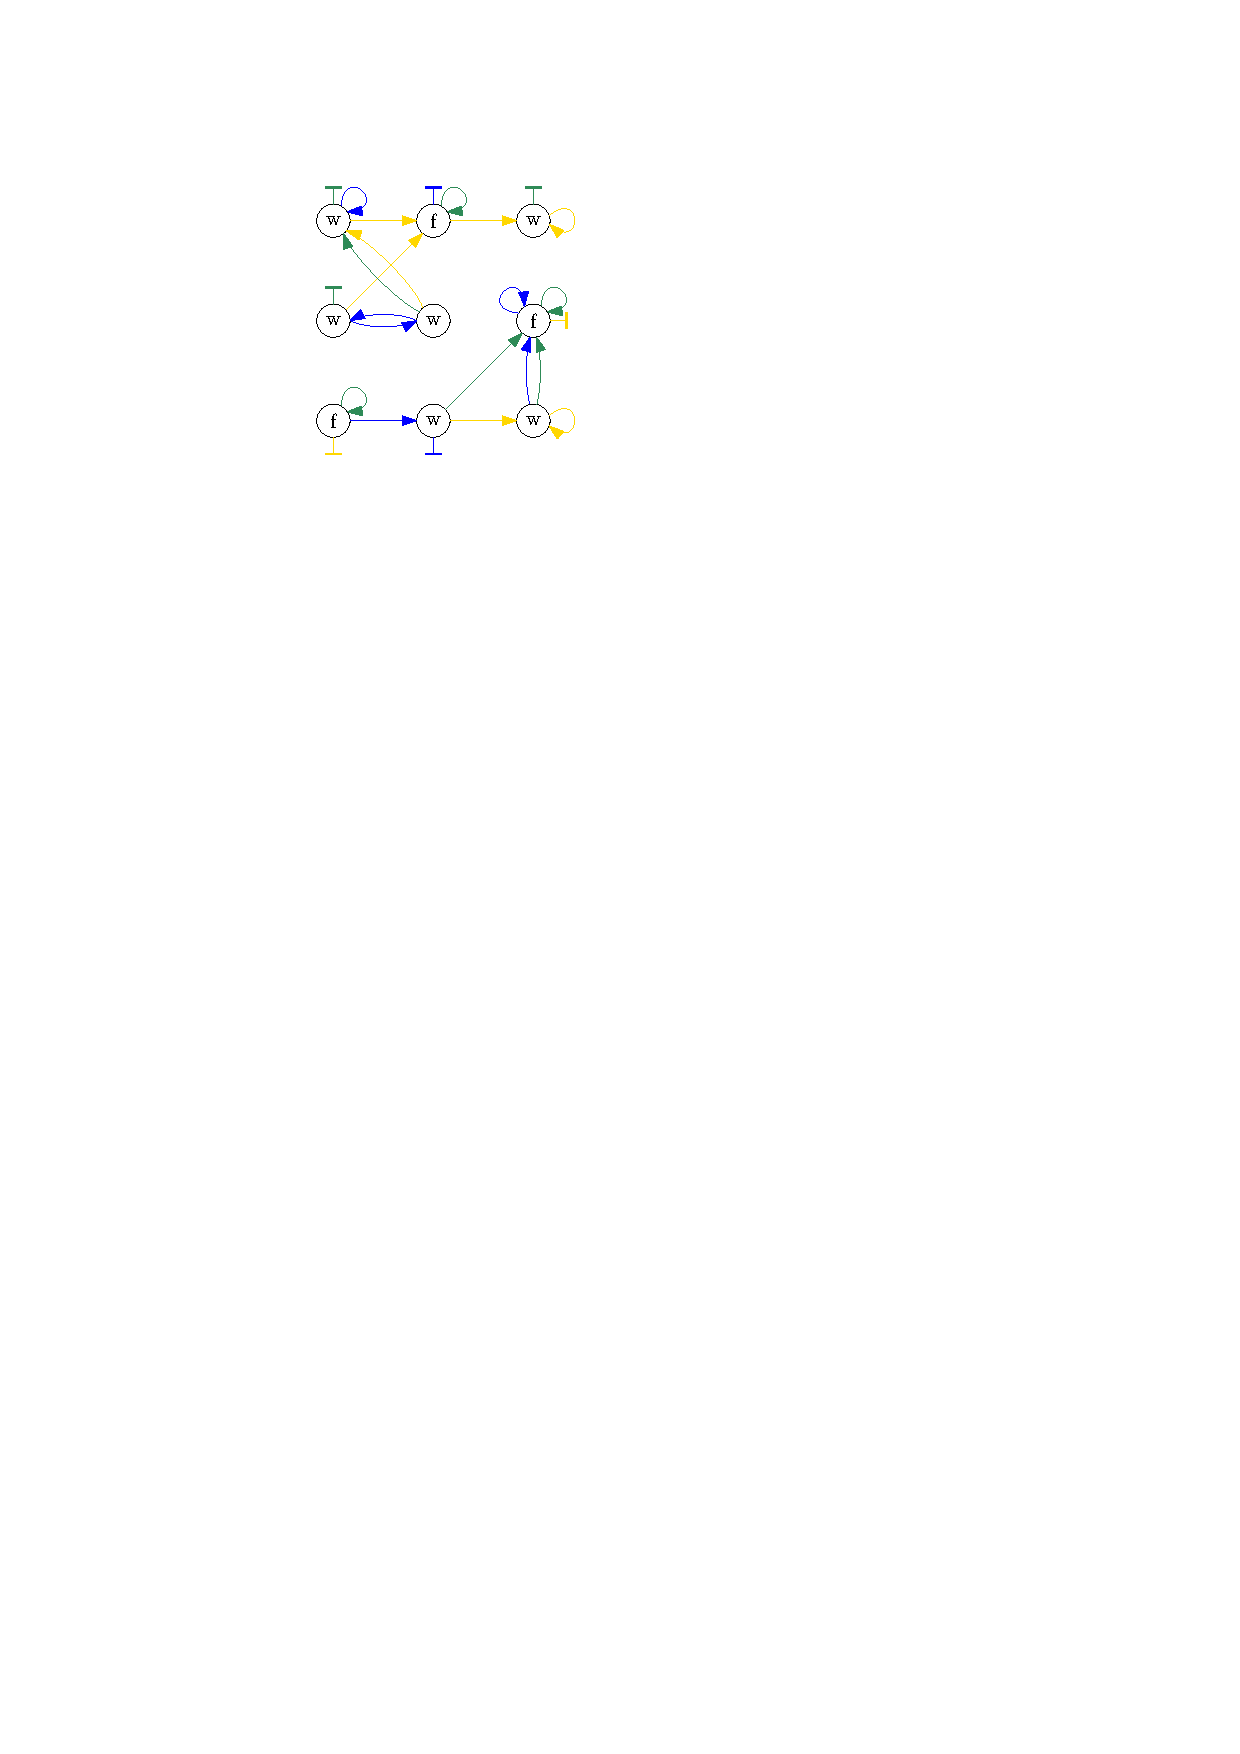
\includegraphics[page=1,width=.4\textwidth]{img/f-combined}
    \caption{Visualisierung der Funktionsverkettung durch $F$}
\end{figure}



\subsubsection{Wie muss ein Fixpunkt aussehen?}

\begin{enumerate}
    \item Für alle Zustände mit Wahrheitswert $\false$ muss der Fixpunkt eine Schleife ($\id$) liefern.
        \begin{figure}[H]
            \centering
            \includegraphics[page=2,width=.15\textwidth]{img/f-combined}
        \end{figure}
    \item Es gibt Zustände mit Wahrheitswert $\true$, die nach endlich vielen Schritten mit $\mathcal{S}$ (gelb) einen Zustand mit Wahrheitswert $\false$ erreichen.
        \begin{figure}[H]
            \centering
            \includegraphics[page=3,width=.6\textwidth]{img/f-combined}
        \end{figure}
    \item Es gibt Zustände mit Wahrheitswert $\true$, die nicht nach endliche vielen Schritten einen Zustand mit Wahrheitswert $\false$ erreichen.
        \begin{enumerate}
            \item $w \to w \to w \to \dots$
\begin{lstlisting}[language=Pascal]
x := 1;
while true do
    x := x + 1
\end{lstlisting}
                \begin{figure}[H]
                    \centering
                    \includegraphics[page=4,width=.6\textwidth]{img/f-combined}
                \end{figure}
                Hier müssen alle Pfeile zum selben Zustand zeigen, egal welcher genau das ist.
            \item  $w_1 \to w_2 \to w_2 \to w_1$
\begin{lstlisting}[language=Pascal]
x := 0;
while x != -1 do
    x := (x + 1) mod 10
\end{lstlisting}
                \begin{figure}[H]
                    \centering
                    \includegraphics[page=5,width=.22\textwidth]{img/f-combined}
                \end{figure}
                Hier müssen ebenfalls alle Pfeile zum selben Zustand zeigen, egal welcher genau das ist.
            \item $w \to w \to w \to \bot$
\begin{lstlisting}[language=Pascal]
x := 1;
while x < 20 do
    x := x + 1;
    if x = 10 then
        while true do skip
    else
        ...
\end{lstlisting}
        \begin{figure}[H]
            \centering
            \includegraphics[page=6,width=.6\textwidth]{img/f-combined}
        \end{figure}
        \end{enumerate}
        Für die Fälle (a) und (b) ist der Fixpunkt also fix aber beliebig (inklusive $\bot$).
\end{enumerate}

\par\bigskip
Das Ergebnis unserer informellen Überlegung ist:
\begin{itemize}
    \item Wir erwarten, dass \emph{immer ein Fixpunkt existiert}.
    \item Ein solcher Fixpunkt ist nicht immer eindeutig. Für Zustände, bei denen die \texttt{while}-Schleife nicht terminiert, kann es ggf. mehrere Möglichkeiten für einen Fixpunkt geben.

        In diesem Fall hätten wir gern den Fixpunkt, der $\bot$ für nicht-terminierende Schleifen liefert.
\end{itemize}


\subsubsection{Fixpunktiteration}

\begin{remark}[Idee]
    Finde die richtigen Fixpunkt durch Fixpunktiteration. Starte mit der Zustandsüberführungsfunktion \[
    f_{\bot} : f_{\bot}(\sigma) = \bot \quad \forall \sigma \in \State
    \]
    welche $F$ wiederholt auf $f_{\bot}$ an, schaue was passiert.

    $\Rightarrow$ Der ``Grenzwert'' ist der gewünschte Fixpunkt.

    Z.\,B. bei (c.a) und (c.b) bleibt die Funktion nach wiederholter Anwendung überall $\bot$.
\end{remark}

\begin{definition}[Fixpunktoperator]
    \begin{align*}
        f_0 & = f_{\bot} \\
        f_n &= F(f_{n-1}) \quad n \geq 1 \\
        \fix(f) & := \lim_{n \to \infty} f_n
    \end{align*}

    Aber wie ist der Grenzwert in diesem Kontext definiert?
\end{definition}

\begin{definition}
    Sei $\mathcal{F} = \{ f \;\vert\; f: \State \to \State \}$ die Menge aller partiellen Zustandsüberführungsfunktionen. Wir definieren auf $\mathcal{F}$ eine Relation $\sqsubseteq$ durch \[
        f \sqsubseteq g :\Longleftrightarrow \forall \sigma, \sigma' \in \State: f(\sigma) = \sigma' \Rightarrow g(\sigma) = \sigma'
        \]
        \dh{} überall, wo $f$ definiert ist, ist auch $g$ definiert und liefert denselben Wert.
\end{definition}

\par\medskip
\begin{example}
    $g_1, g_2, g_3, g_4 : \State \to \State$
    \begin{align*}
        g_1(\sigma) & = \sigma \quad \forall \sigma \in \State \\
        g_2(\sigma) & = \begin{cases}
            \sigma & \text{falls } \sigma(x) \geq 0 \\
            \bot & \text{sonst} \\
        \end{cases} \\
        g_3(\sigma) & = \begin{cases}
            \sigma & \text{falls } \sigma(x) \leq 0 \\
            \bot & \text{sonst} \\
        \end{cases} \\
        g_4(\sigma) & = \begin{cases}
            \sigma & \text{falls } \sigma(x) = 0 \\
            \bot & \text{sonst} \\
        \end{cases} \\
    \end{align*}
    Behauptung:
    \begin{align*}
        g_4 \sqsubseteq g_2 \sqsubseteq g_1 \\
        g_4 \sqsubseteq g_3 \sqsubseteq g_1 \\
        g_4 \sqsubseteq g_1 \tag{*}
    \end{align*}
    $(*)$ folgt aus Transivität da die Relation eine Ordnungsrelation ist, aber das haben wir noch nicht bewiesen.

    Jedoch sind $g_2$ und $g_3$ nicht vergleichbar.
\end{example}

\par\bigskip
\begin{remark}[Fakt]
    $\sqsubseteq$ ist eine Ordnungsrelation auf $\mathcal{F}$. Das bedeutet, sie ist
    \begin{itemize}
        \item reflexiv: $f \sqsubseteq f$
        \item transitiv: $f \sqsubseteq g \wedge g \sqsubseteq h \Rightarrow f \sqsubseteq h$
        \item antisymmetrisch: $f \sqsubseteq g \wedge g \sqsubseteq f \Rightarrow f = g$
    \end{itemize}

    $(\mathcal{F}, \sqsubseteq)$ ist eine Halbordnung (poset bzw. partially ordered set).
\end{remark}

\par\medskip
\begin{definition}
    Ein Element $f \in \mathcal{F}$ heißt \emph{Minimum}, falls für alle $g \in \mathcal{F}$ gilt \[
    f \sqsubseteq g
    \]
\end{definition}

\begin{remark}[Beobachtungen]
    Im Allgemeinen, muss es kein Minimum in einem poset geben (\zb{} unendliche Ordnung oder mehrere nicht vergleichbare minimale Elemente). Wenn ein Minimum existiert, dann ist es eindeutig (wegen Antisymmetrie).

    Aber $(\mathcal{F}, \sqsubseteq)$ hat ein Minimum und zwar $f_{\bot}$.
\end{remark}


